%!TEX root = ../main.tex

\chapter{Visualization}
Full three-dimensional spatial stochastic simulations can be difficult to analyze. To simplify the process, StochSS has built in three different methods for visualization of spatial models.

\section{Surface Renderings with Domain Clipping}

By default, spatial stochastic simulations are rendered as shown in Figure \ref{surface}. These are surface renderings, but the simulations are volumetric. To see inside the volume, StochSS allows slicing the mesh in half along one axis with a plane and only rendering one of the resultant halves. This is shown in Figure \ref{clipx}

\begin{figure}[!ht]
  \centering
    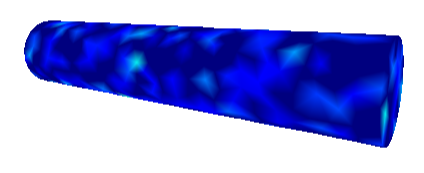
\includegraphics[width=0.5\textwidth]{Vis/surface}
  \caption{ Surface rendering of cylindrical domain. The actual stochastic simulation is run on the dual of the shown mesh, so the color at each node corresponds to the concentration in the corresponding voxel of the dual mesh. Colors are interpolated linearly between nodes. The color scale is not shown for brevity. }
  \label{surface}
\end{figure}

\begin{figure}[!ht]
  \centering
    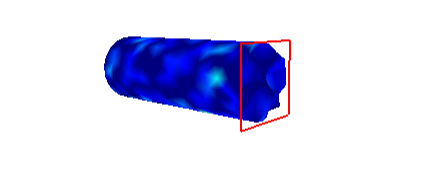
\includegraphics[width=0.5\textwidth]{Vis/clipx}
  \caption{ Surface rendering of cylindrical domain clipping along the X dimension. It is now possible to see concentrations of voxels inside the cylinder. }
  \label{clipx}
\end{figure}

\section{Colorized Wireframe Meshes}

The second rendering type is similar to the first, but instead of rendering surfaces only edges are rendered (see Figure \ref{wireframe}). The colorization is the same, it is just ideally easier to see inside the mesh. Similarly to the surface rendering the wireframe renderings can be clipped to get a clearer view of what is happening inside the volume. See Figure \ref{clipy} for a demonstration of clipping a mesh in the Y dimension.

\begin{figure}[!ht]
  \centering
    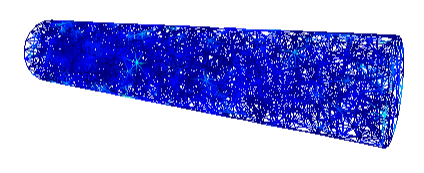
\includegraphics[width=0.5\textwidth]{Vis/wireframe}
  \caption{ Wireframe rendering of cylindrical domain. The colors are handled similarly to in Figure \ref{surface}. }
  \label{wireframe}
\end{figure}

\begin{figure}[!ht]
  \centering
    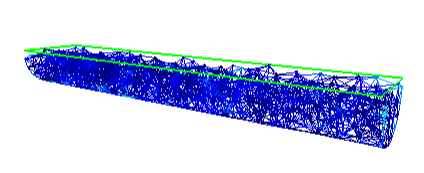
\includegraphics[width=0.5\textwidth]{Vis/clipy}
  \caption{ Wireframe rendering of cylindrical domain clipped in the Y direction. }
  \label{clipy}
\end{figure}

\section{Volume Rendering}

The final rendering StochSS offers is a volume rendering (Figure \ref{fig:volume}). It uses a basic ray-tracing implementation following the one in \cite{congote}.

\begin{figure}[!ht]
  \centering
    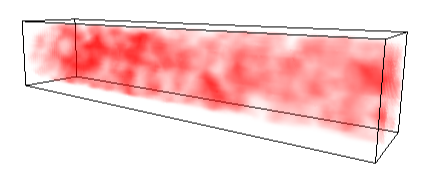
\includegraphics[width=0.5\textwidth]{Vis/volume}
  \caption{ This is the volume rendering of the same data shown above. The idea behind volume rendering is to color darkly areas with high concentrations and leave volumes with low concentrations transparent. The transparency makes it possible to see inside a volume rendering, and so the slicing as shown in the surface and wireframe renderings is not used. }
  \label{fig:volume}
\end{figure}

\section{Visualization in Interactive Jupyter Notebook}

In many projects the need to perform custom postprocessing and visualization will eventually arise. To facilitate this process, StochSS offers the possibility to export a Jupyter Notebook template, which reads the output and plots the average populations of the species. The user can then customize the Notebook to perform the required postprocessing and plotting.

To access this function, simply click \textbf{Analyze using Interactive Notebook} on the \textbf{Job Summary} page. Figure \ref{vis-jupyter} shows the default template.

For documentation and tutorials on Jupyter Notebooks, see http://jupyter.org.

\begin{figure}[!ht]
\centering
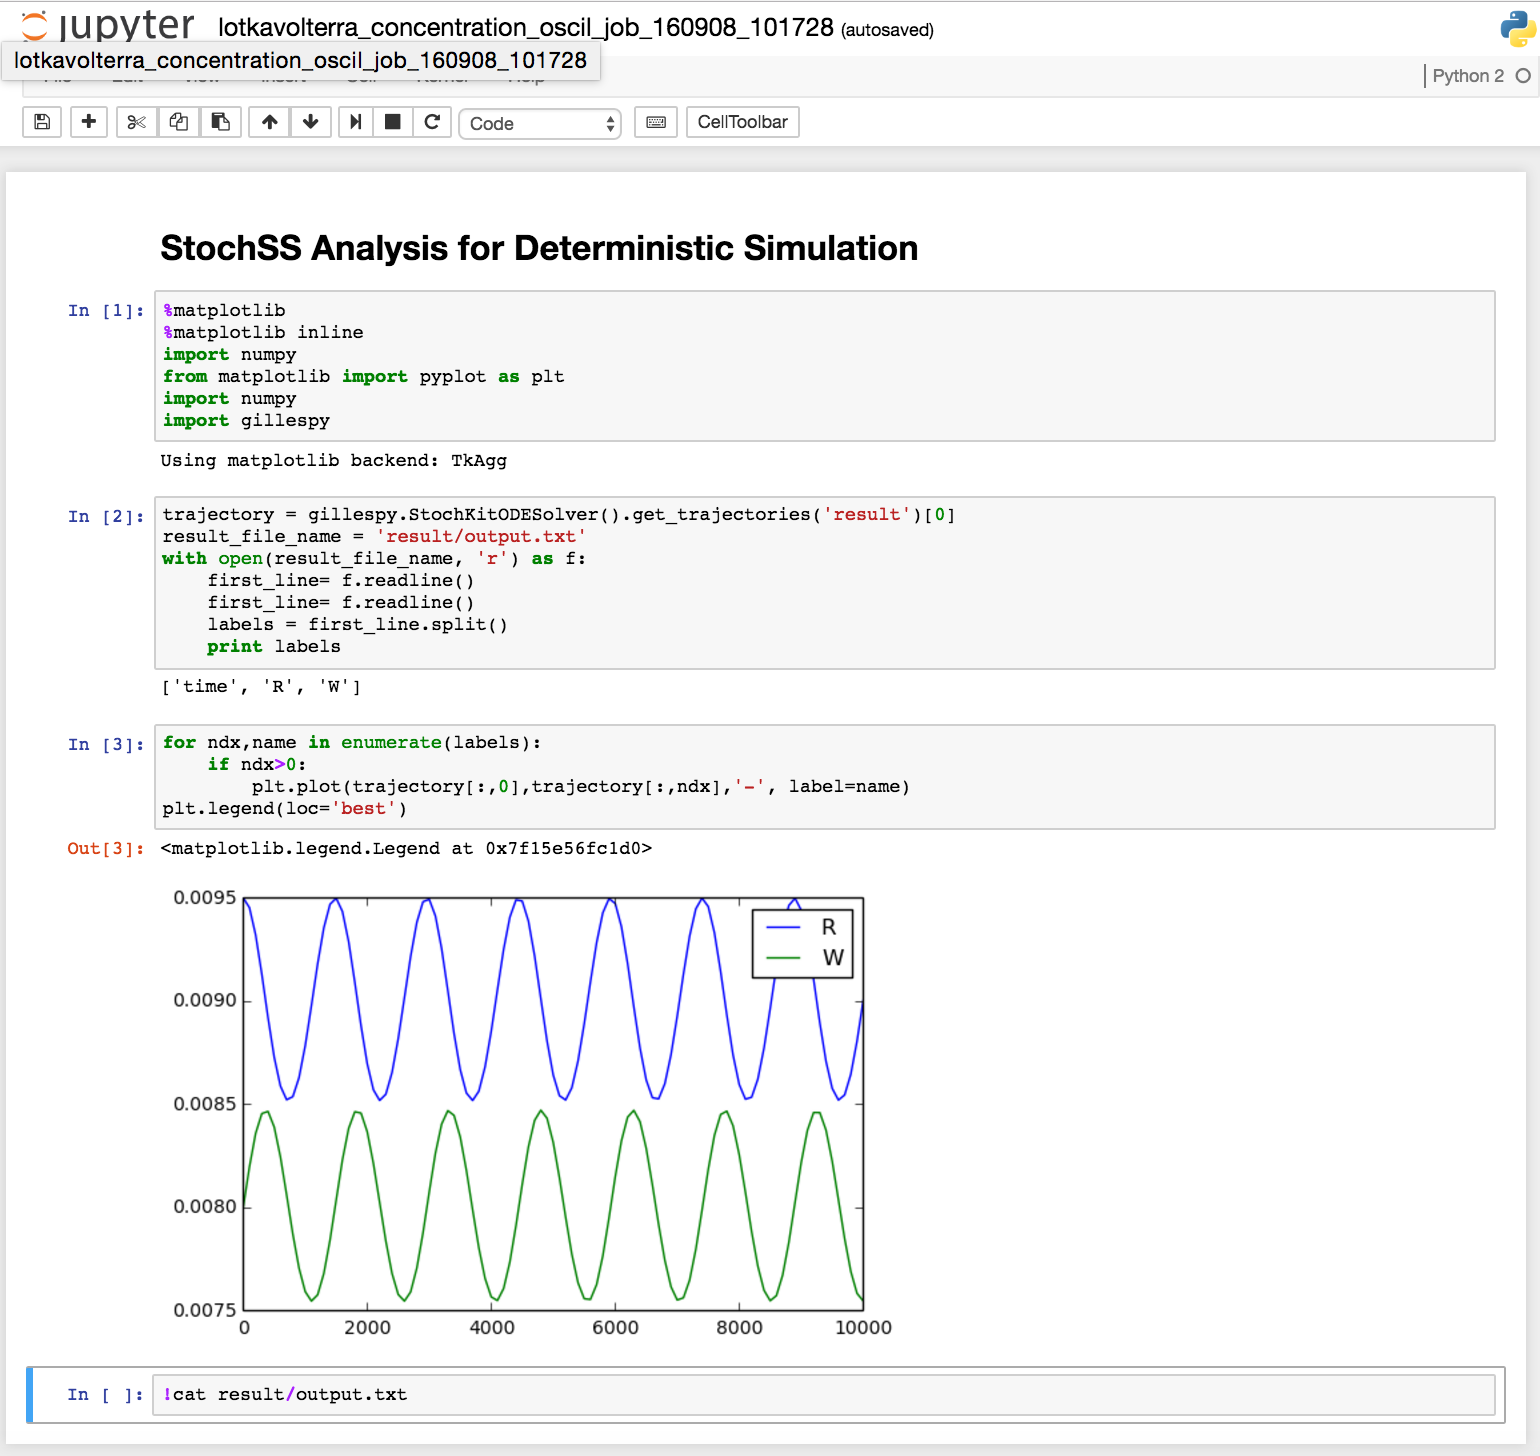
\includegraphics[width=0.8\textwidth]{Vis/vis-jupyter.png}
\caption{\label{vis-jupyter}Default Notebook for custom postprocessing.}
\end{figure}


